% Session 4 -- the Landau fans: Schroedinger levels linear in B, Dirac levels as sqrt(B), with an exact zero mode.
% Placement: sec. "Landau levels of Dirac electrons", after equation (4.7).
% Rendered by figures/blender/s04f04_ladders.py, labels in figures/overlays/s04f04_ladders.tex.
\begin{aqmfigure}{fig:s04:ladders}{The same magnetic field with two dispersions gives two completely
different ladders, drawn here as functions of the field. (a) Schr\"odinger electrons give the
harmonic-oscillator spectrum (4.6), where every level is a constant $\hbar\omega_c=\hbar B/m$ above
the one below it, so every level is a straight line through the origin and the whole ladder grows
linearly in $B$. (b) Dirac electrons give the square root of that spectrum, equation (4.7). The
levels come closer together as $\sqrt{n}$, they come in a particle-hole symmetric pair for every
$|n|\ge1$, and the overall scale grows only as $\sqrt{B}$. This is still enough to put the level
spacing of graphene about two orders of magnitude above the one of a GaAs quantum well at the same
field. The $n=0$ level is the qualitatively new feature. It stays at exactly zero energy for every
field strength, which is the flat line, because it is the only solution with no partner in the other
spinor component. The translucent plane at the field $B_0$ cuts each fan, and the short rods where
it cuts are the ladder of levels at that field, so the ladder at a fixed field is the vertical cut
through the fan. The two vertical scales are independent of each other, since what we compare is the
pattern of spacings and not the absolute energies.}
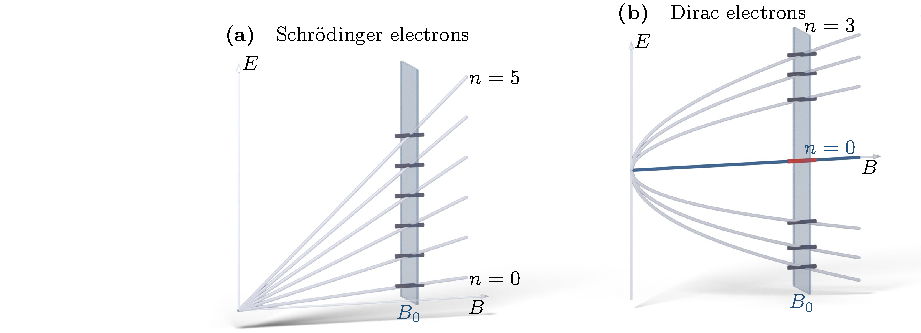
\includegraphics{figures/pdf/s04f04_ladders.pdf}
\end{aqmfigure}
